\documentclass[12pt]{article}
\usepackage{pgfplots}
\usepgfplotslibrary{groupplots}
\usepackage{multirow}
\pgfplotsset{compat=1.18}
\usepackage{graphicx}
\usepackage{amsmath} 
\usepackage{ragged2e}
\usepackage{amssymb}
\usepackage{float}
\usepackage{mathabx}
\usepackage{mathtools}
\usepackage{tikz}
\usepackage{tikz-3dplot}
\usepackage{caption}
\usepackage[makeroom]{cancel}
\usepackage{biblatex} 
\usepackage{amsfonts}
\usepackage{url}
\usepackage{gensymb}
\usepackage{mathrsfs}
\usepackage{titling}
\usepackage{circuitikz}
\addbibresource{citations.bib}
\newcommand{\subtitle}[1]{
  \posttitle{
    \par\end{center}
    \begin{center}\large#1\end{center}
    \vskip0.5em
  }
}
\newtheorem{theorem}{Theorem}
\newtheorem{definition}{Definition}

\title{The Laplacian as a Spatial Low-Pass Filter: An Intuitive Derivation of the Poisson Kernel}
\author{Giovani Mendes Crepaldi}
\date{October 2026}

\begin{document}

\maketitle
\section{Disclaimer}
This independent study is not sufficiently mathematically rigorous, and should only be read as a complement to intuition or introduction on the subject.

\section{Definitions}
\begin{definition}
    \text{The Fourier Transform of a function }\(f(x)\)\text{ is denoted as:}
\[
\mathscr{F}(\xi)=\hat{f}(\xi):=\int_{\mathbb{R}^{n}}f(x)e^{-2\pi ik\xi}dx
\]
\end{definition}
\begin{definition}
    \text{The inverse Fourier Transform of a function }\(f(x)\)
    \text{is denoted as:}
\[
f(x) :=\frac{1}{2\pi} \int_{\mathbb{R}^{n}} \hat{f}(\xi) e^{2\pi i x \xi} \, d\xi,
\]
\begin{definition}
    A convolution of two functions f(x) and g(x) is given by:
\[
(f*g)(x)=h(x):=\int_{\mathbb{R}}f(\tau)g(x-\tau)d\tau
\]
\end{definition}
\begin{theorem}
    Let \((f,g)\) be functions in a space where Fubini's theorem is valid.
    Let h(x) be the convolution \((f*g)(x)\). 
    Then:    
\[
    \hat{h}(\xi)=\hat{f}(\xi) \hat{g}(\xi)
\]  
\end{theorem}

Firstly, we substitute:
\[
    \hat{h}(\xi)=\int_{\mathbb{R}}h(x)e^{-2\pi ix\xi}dx
\]
By definition:
    
\[
\int_{\mathbb{R}}h(x)e^{-2\pi ix\xi}dx=\int_{\mathbb{R}}\int_{\mathbb{R}}f(\tau)g(x-\tau)e^{-2\pi ix\xi}d\tau dx
\]
By Fubini's theorem:
\[
\int_{\mathbb{R}}\int_{\mathbb{R}} f(\tau)g(x-\tau)e^{-2\pi ix\xi}d\tau dx=\int_{\mathbb{R}}(\int_{\mathbb{R}}g(x-\tau)e^{-2\pi ix\xi}dx)f(\tau)d\tau
\]
From a simple u substitution:
\[
\int_{\mathbb{R}}(\int_{\mathbb{R}}g(x-\tau)e^{-2\pi ix\xi}dx)f(\tau)d\tau=\hat{g}(\xi)\int_{\mathbb{R}}f(\tau)e^{-2\pi i\xi \tau}d\tau=\hat{f}(\xi)\hat{g}(\xi)
\]    
\end{definition}

\section{Introduction: Definitions, physical interpretations and the problem}
The Laplacian equation for a 2 dimensional body is defined by \(\nabla ^2 f\). Formally, it represents the divergence of the gradient of \(f\), but this definition is not really intuitive(at least for me), so I like to think of it from another perspective.
\newline
Say we have a hot bar of metal with temperature distribution T(t,x), so the temperature varies as we walk on the x-axis, but it also changes when time passes.
Now, think about what happens if we take a couple of discrete points of this bar of length L:
\begin{center}
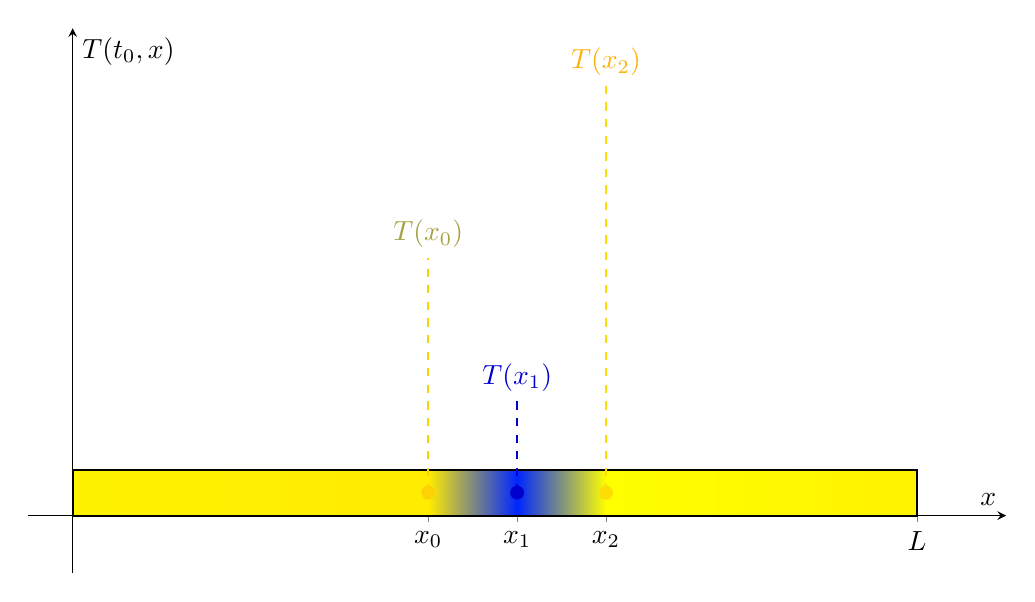
\begin{tikzpicture}
  \begin{axis}[
    width=14cm,
    height=8.5cm,
    axis lines=middle,
    xmin=-0.5, xmax=10.5,
    ymin=-1, ymax=8.5,
    xlabel={$x$},
    ylabel={$T(t_0,x)$},
    xtick={4.0, 5.0, 6.0, 9.5},
    xticklabels={$x_0$, $x_1$, $x_2$, $L$},
    ytick=\empty,
    enlargelimits=false
  ]

    \shade[shading=axis, left color=yellow!90!orange, right color=yellow!85!orange] (0,0) rectangle (4.0,0.8);
    \shade[shading=axis, left color=yellow!85!orange, right color=blue!85!cyan] (4.0,0) rectangle (5.0,0.8);
    \shade[shading=axis, left color=blue!85!cyan, right color=yellow!100!orange] (5.0,0) rectangle (6.0,0.8);
    \shade[shading=axis, left color=yellow!100!orange, right color=yellow!90!orange] (6.0,0) rectangle (9.5,0.8);

    \draw[thick, black] (0, 0) rectangle (9.5, 0.8);

    \draw[dashed, yellow!70!orange, thick] (4.0, 0.4) -- (4.0, 4.5);
    \node[above, yellow!60!black] at (4.0, 4.5) {$T(x_0)$};
    \fill[yellow!70!orange] (4.0, 0.4) circle (2.5pt);

    \draw[dashed, blue!80!black, thick] (5.0, 0.4) -- (5.0, 2.0);
    \node[above, blue!80!black] at (5.0, 2.0) {$T(x_1)$};
    \fill[blue!80!black] (5.0, 0.4) circle (2.5pt);

    \draw[dashed, yellow!90!red, thick] (6.0, 0.4) -- (6.0, 7.5);
    \node[above, yellow!70!red] at (6.0, 7.5) {$T(x_2)$};
    \fill[yellow!90!red] (6.0, 0.4) circle (2.5pt);

  \end{axis}
\end{tikzpicture}
\end{center}

 For simplicity, let  $x_0, x_1, x_2$ be such that $x_1=\frac{x_0+x_1}{2}$ that is, the space between the neighboring points is the same $\Delta x$, we define $\\ \delta T_1 = T(x_1) - T(x_0) \\ \delta T_2 = T(x_2) - T(x_1) $, Then, if we want to calculate the rate of change in its proper reference:
 \[m_1 = \frac{\delta_1}{\Delta x} = \frac{T(x_1) - T(x_0)}{\Delta x}\\
 m_2 = \frac{\delta_2}{\Delta x} = \frac{T(x_2) - T(x_1)}{\Delta x}\]
 that means, intuitively, how fast(velocity) $T(x_1)$ gets in relation to its reference.
 But if we have an answer for how fast something is, its only logical to ask its acceleration, that is, the rate of change of the rate of change(or the curvature),(the final formula is just a representation of the discrete laplacian for 1D, we won't really use it)
 \[
a= \frac{m_2 - m_1}{\Delta x} = \frac{\frac{T(x_2) - T(x_1)}{\Delta x} - \frac{T(x_1) - T(x_0)}{\Delta x}}{\Delta x} = \frac{T(x_0) - 2T(x_1) + T(x_2)}{(\Delta x)^2}
 \]
 But if we describe the acceleration, that relates directly to its second partial derivative when we make \(\Delta x\) infinitesimally small:
 \[\frac{\partial ^2T}{\partial x^2}\approx \alpha\frac{m_2-m_1}{(\Delta x)^2}\]
\(\alpha\) is only a constant that relates to how heat dissipates on that material.
Remember,
\[
m=\frac{\delta}{\Delta x}
\]
when \(\Delta x\) is infitesimaly small
\[
m\approx \frac{\partial T}{\partial x}
\] 
In its corresponding index for m and T.

That acceleration or curvature of how quickly the system "settles down" locally is exactly the laplacian operator.
\[\alpha\nabla^2T=\frac{\partial^2T}{\partial x^2}\]
Of course we only semi-proved it for one dimension, but it is intuitive to think about for at least 3 dimensional spaces, although we will only think about 2 dimensional spaces in this study.
Then, when extending this line of thinking, imagining a sheet of heated metal, this acceleration in which the space settles down, now accounting for the possibility of 2 dimensions dissipating heat in accordance to its neighbor:
\[\nabla ^2 T(x,y)=\frac{\partial^2T}{\partial x^2}+\frac{\partial^2T}{\partial y^2}\]
From now on, we will use the notation:
\[\frac{\partial u}{\partial x}=u_{x}\text { Similarly, } \frac{\partial^2u }{\partial x^2}=u_{xx}\]
We will look firstly at partial differential equations where \(\nabla^2f=0\), in one dimension, it means that the rate of change between the points is a constant, which means the acceleration is zero. 
But on 2 dimensions, it means that, the curvature in x is always compensated by the curvature in y, if the function is increasing on x, it must be decreasing on y on its neighboring points, and vice-versa.
Now, let me take a step back, and introduce why this matters on an electrical engineering perspective. the electrical field E, always points in the direction where the potential gets lower.
\begin{center}
    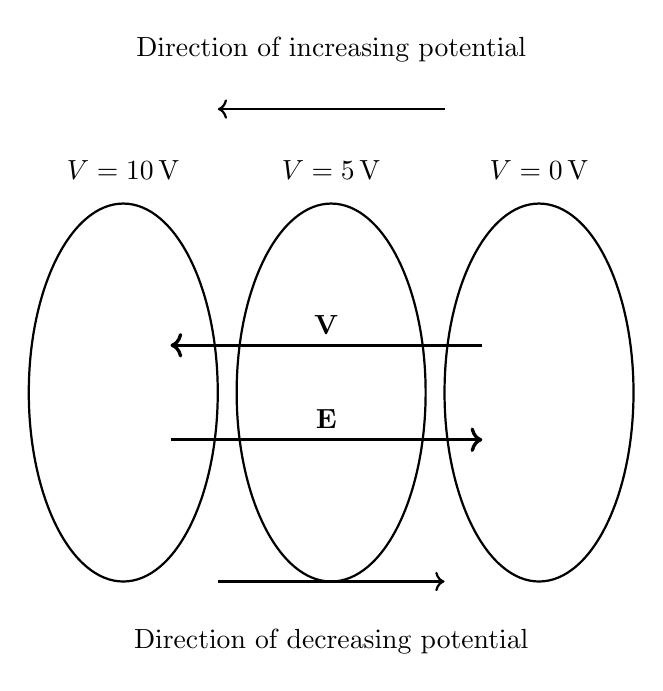
\begin{tikzpicture}[scale=1.2]

    
    \draw[thick] (0,0) ellipse (1.0 and 2.0);
    \draw[thick] (2.2,0) ellipse (1.0 and 2.0);
    \draw[thick] (4.4,0) ellipse (1.0 and 2.0);

    
    \node at (0,2.35) {$V=10\,\mathrm{V}$};
    \node at (2.2,2.35) {$V=5\,\mathrm{V}$};
    \node at (4.4,2.35) {$V=0\,\mathrm{V}$};

    
    \draw[->, very thick] (0.5,-0.5) -- (3.8,-0.5)
        node[midway, above] {$\mathbf{E}$};
    \draw[->, very thick] (3.8,0.5) -- (0.5,0.5)
        node[midway, above] {$\mathbf{V}$};

    
    \node[below] at (2.2,-2.4)
        {Direction of decreasing potential};
    \node[above] at (2.2,3.4)
        {Direction of increasing potential};

    
    \draw[->, thick] (1.0,-2.0) -- (3.4,-2.0);
    \draw[->, thick] (3.4,3)--(1.0,3) ;

\end{tikzpicture}

\end{center}
This makes sense when you think about field lines, a particle with a positive charge has an electrical field pointing away from the particle, say the particle has tension \(V_0\) and using the convention that \(V_\infty =0\), if \(V_0\) if the electrical field, points away from a positive charge, in the direction of a "point" that has no tension, it can only be that it walks on the negative path from which the tension grows the fastest. Mathematically, this just means:
\[E=-\nabla V\]
Now, if we think about how the electrical field spreads from a point, which I think intuitively of sinks and sources, just like liquids flow outwards, and sinks pulls liquid in, the same happens to charges(sinks are negative charges and sources are positive charges), that is represented mathematically by its divergence, now, how much can the electrical field(liquid) flow outwards? It depends on its "viscosity", back to the electrical field, since electrical fields don't have viscosity, the only other thing that can get in the way of the field are other charges. More specifically, the charge density \(\rho\). Then:
\[\nabla E\propto \rho\]
even more specifically:
\[\nabla E=\frac{\rho}{\epsilon_0}\]
if we substitute \(E=-\nabla V\):
\[-\nabla^2 V=\frac{\rho}{\epsilon_0}\]
In a region free of other charges(like a relative vacuum, for example)(\(\rho=0\)):
\[\nabla^2V=0\]
This means that, if we have no outside charges, the laplacian is zero, therefore the function is harmonic, the function being harmonic brings forth a bunch of useful theorem, but I think that the most helpful result to understanding the laplacian(=0), is that harmonic functions have no spontaneous uniqueness(Dirichlet's problem). And that it may be used as a low-pass filter, we will see why that happens shortly, but its useful to visualize this now.
\newline 
To set an example,
look at the graph \(z=\cos(cx)e^{-cy}\) for different c values:
\[c=1\]
\begin{figure}[H]
\centering
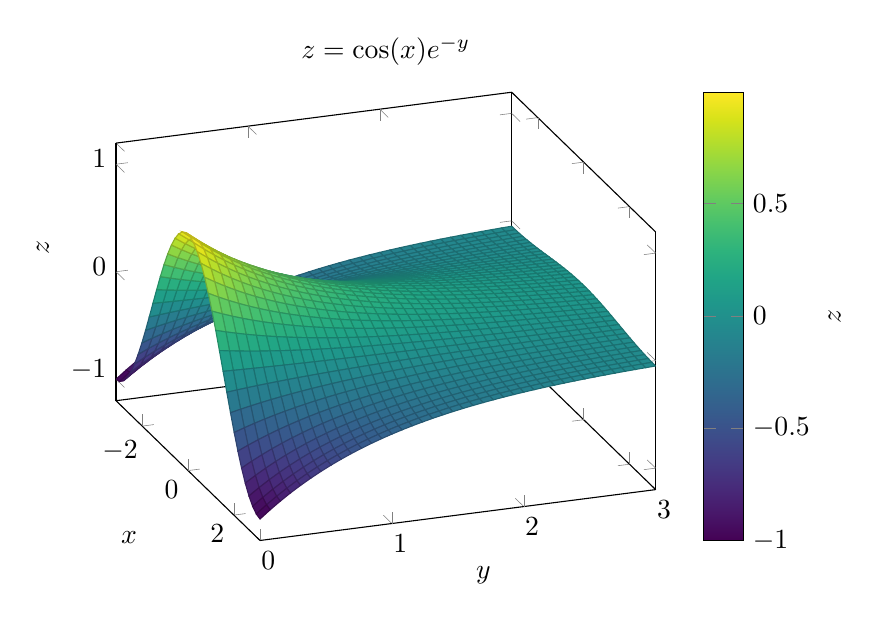
\begin{tikzpicture}
\begin{axis}[
    title={$z = \cos(x)e^{-y}$},
    xlabel={$x$},
    ylabel={$y$},
    zlabel={$z$},
    colormap/viridis,
    view={70}{30},
    colorbar,
    colorbar style={
        ylabel={$z$}
    }
]
\addplot3[
    surf,
    domain=-3.14159:3.14159,
    domain y=0:3,
    samples=40,
    samples y=40,
    trig format=rad
] {cos(x)*exp(-y)};
\end{axis}
\end{tikzpicture}
\caption{3D surface plot of $z=\cos(cx)e^{-cy}$ for c=1.}
\label{fig:cos_exp_surface}
\end{figure}
\[c=10\]
\begin{figure}[H]
\centering
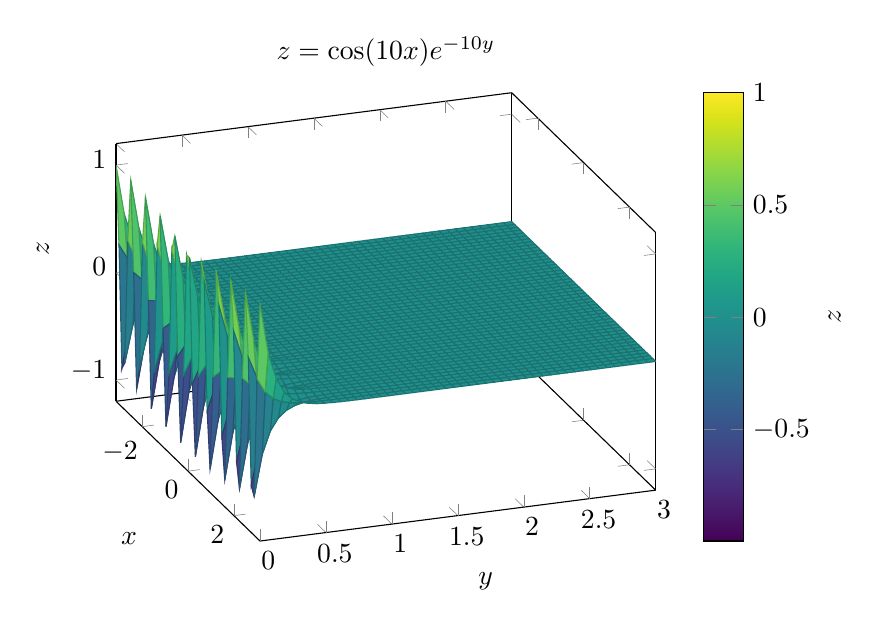
\begin{tikzpicture}
\begin{axis}[
    title={$z = \cos(10x)e^{-10y}$},
    xlabel={$x$},
    ylabel={$y$},
    zlabel={$z$},
    colormap/viridis,
    view={70}{30},
    colorbar,
    colorbar style={
        ylabel={$z$}
    }
]
\addplot3[
    surf,
    domain=-3.14159:3.14159,
    domain y=0:3,
    samples=50,
    samples y=50,
    trig format=rad
] {cos(10*x)*exp(-10*y)};
\end{axis}
\end{tikzpicture}
\caption{3D surface plot of $z = \cos(10x)e^{-10y}$ in the original scale.}
\label{fig:cos_exp_scaled}
\end{figure}

As you can see, higher frequencies tend to zero quicker than lower frequencies. Meaning that the Laplacian may be used as a low-pass filter. To formalize this, and for better intuition, we must derive a general solution for the 2D laplacian given the spacial countour conditions that apply to voltage analysis.

\section{General Solution for \(\nabla^2U=0\)}
\begin{theorem}
    The general solution for the 2D laplacian for contour conditions \(u(x,0)=f(x)\) and \(\lim_{y\rightarrow \infty} u(x,y)=0\), \(\nabla ^2u=0\) is a convolution of the contour condition \(f(x)\) with the Kernel Poisson.
    \[u(x,y)=P(x,y)*f(x)\]
\end{theorem}
"Proof":
\[
u_{xx}+u_{yy}=0
\]
We do a Fourier transform of the system in \(x\mapsto \xi\), and since derivative in respect to other variables is linear, and using the derivative property of the Fourier transform:
\[
(i\xi)^2\hat{u}(\xi,y)+\frac{\partial^2 }{\partial y^2}\hat{u}(\xi,y)=0
\]
Therefore, we have an equivalent ODE:
\[
\hat{u}_{yy}(\xi,y)-\xi^2\hat{u}(\xi,y)=0
\]
The general solution for this EDO:
\[\hat{u}(\xi,y)=A(\xi)e^{\mid\xi\mid y}+B(\xi)e^{-\mid \xi \mid y}\]
Since \(\lim_{y\rightarrow\infty} u(x,y)=0\rightarrow \lim_{y\rightarrow\infty}\hat{u}(\xi,y)=0\), we apply this contour condition:
\[
\lim_{y\rightarrow \infty}A(\xi)e^{\mid\xi\mid y}+B(\xi)e^{-\mid \xi \mid y}=0
\]
But, in the second term we have a negative exponential:
\[\lim_{y\rightarrow \infty}B(\xi)e^{-\mid \xi \mid y}=0\]
Therefore:
\[\lim_{y\rightarrow \infty}A(\xi)e^{\mid\xi\mid y}=0\Leftrightarrow A(\xi)=0 \therefore \]
\[\hat{u}(\xi,y)=B(\xi)e^{-\mid \xi \mid y}\]
From the contour condition \(u(x,0)=f(x)\rightarrow\hat{u}(\xi,0)=\hat{f}(\xi)\):
\[\hat{u}(\xi,0)=B(\xi)\rightarrow B(\xi)=\hat{f}(\xi)\]
\[\hat{u}(\xi,y)=\hat{f}(\xi)e^{-\mid \xi \mid y}\]
This result may help understand the low-pass property, as we increase the frequency, the function decreases by a factor of a negative exponential.
\newline
From this point, we can use the previously demonstrated convolution theorem, to point out that:
\[
u(x,y)=f(x)*g(x,y)
\]
Then, following the definition:
\[
g(x,y) =\frac{1}{2\pi} \int_{\mathbb{R}} e^{-\mid \xi \mid y} e^{2\pi i x \xi} \, d\xi,
\]
Solving this integral yields the Poisson Kernel:
\[
P(x,y)=\frac{1}{\pi}\frac{y}{y^2+x^24\pi^2}
\]
We can think of \(4\pi^2\) as a constant \(c\):
\[
P(x,y)=\frac{1}{\pi}\frac{y}{y^2+x^2c}
\]
Therefore:
\[
u(x,y)=P(x,y)*f(x)
\]
As you might have already noticed, the denominator of this kernel looks a lot like cartesian representation of a circle \(x^2+y^2\) (If we mess around with the definition of the Fourier transform a bit, c disappears and we are left with only that).
Take a look at what it looks like plotted:
\begin{figure}[H]
    \centering
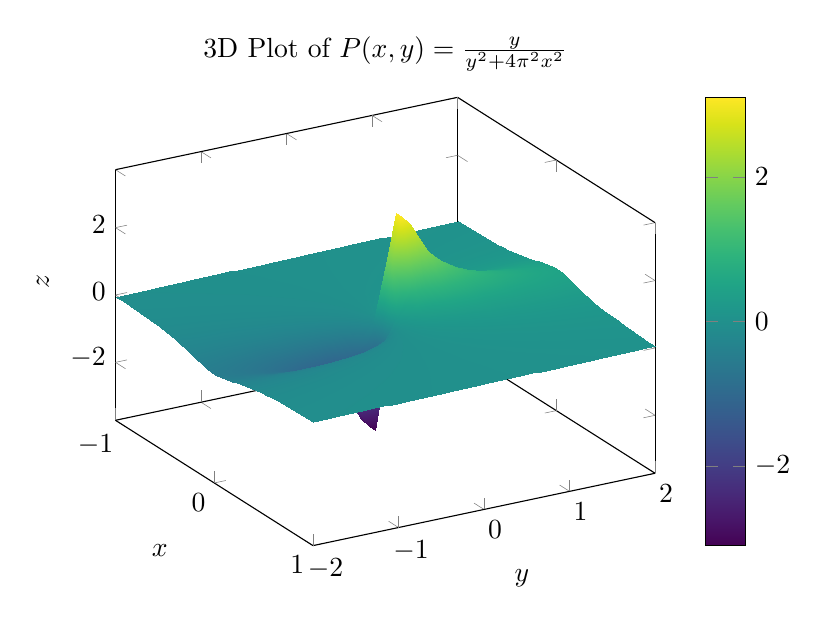
\begin{tikzpicture}
    \begin{axis}[
        title={3D Plot of $P(x,y) = \frac{y}{y^2 + 4\pi^2 x^2}$},
        xlabel={$x$},
        ylabel={$y$},
        zlabel={$z$},
        domain=-1:1,
        domain y=-2:2,
        samples=40,
        samples y=40,
        view={60}{30},
        colormap/viridis,
        colorbar,
        unbounded coords=discard
    ]
        \addplot3[
            surf,
            shader=interp
        ] { y / (y^2 + 4 * (pi^2) * x^2) };
        
    \end{axis}
\end{tikzpicture}
\end{figure}

Since We are only concerned with the \(y\geq 0\) portion of the graph, focus only on the peak at y=0 forward. The intuition for this result is that it closely relates to how waves dissipate physically.
\begin{figure}[H]
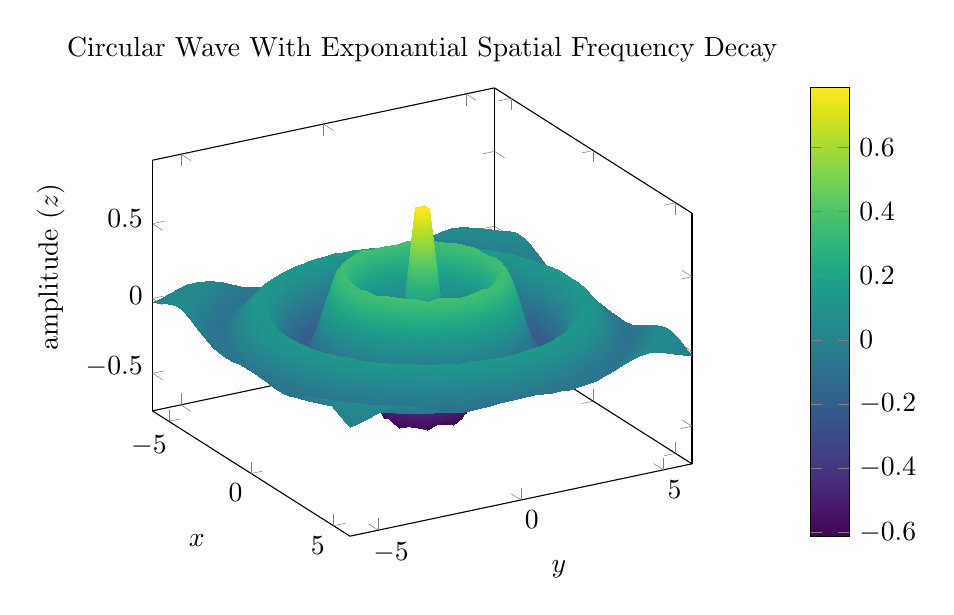
\begin{tikzpicture}
\begin{axis}[
    title={Circular Wave With Exponantial Spatial Frequency Decay},
    xlabel={$x$},
    ylabel={$y$},
    zlabel={amplitude ($z$)},
    domain=-6:6,
    domain y=-6:6,
    samples=40,  
    samples y=40,
    view={60}{30}, 
    colormap/viridis,
    colorbar,
    unbounded coords=discard
]
\addplot3[
    surf,
    shader=interp
] {exp(-sqrt(x^2 + y^2)*0.4) * cos(deg(sqrt(x^2 + y^2)*2.5))};

\end{axis}
\end{tikzpicture}
\end{figure}
An input wave, let's say a ripple in the water, as it dissipates from it's original location, it follows a circular path as its amplitude goes down to zero, or, on the frequency domain, it's spatial frequency decays exponentially.
Water ripples can be modelled by a convolution of the initial ripple conditions, that is, what caused the ripples? Was it a fast or a slow motion that created it? Notably, Water can act as a low-pass filter.
\newline
A curiosity about this phenomenon, this is the reason that, when speaking underwater, the high-frequency sound waves like the consonants "s" or "t", are quickly blocked by the water and lose energy very quick, whereas low-frequency vowels can dissipate better(or for longer) on the water.

\end{document}
